\chapter{Results}
\label{chp:R}

%%%%%%%%%%%%%%%%%%%%%%%%%%%%%%%%%%%%%%%%%%%%%%%%%%%%%%%%%%%%%%%%%%%%%%%

This chapter illustrates results obtained from sample simulations of large populations of units according to the outlined unit generation methods in Section~\ref{ssec:uapg} and the analysis approaches outlined in Section~\ref{ssec:aa}. The software pipeline described in Section~\ref{sec:SW} was used to generate the units and obtain the results.

\section{Monte Carlo Analysis}

Table~\ref{tab:defpar} contains the default parameter values. Unless specified otherwise, parameters were set to the values in Table~\ref{tab:defpar}.

% Please add the following required packages to your document preamble:
% \usepackage{booktabs}
\begin{table}[H]
\centering
\caption{Default simulation parameter values}
\label{tab:defpar}
\begin{tabular}{@{}lc@{}}
\toprule
\multicolumn{1}{c}{\textbf{Parameter}} & \textbf{Value}                 \\ \midrule
\textit{n\_u}                          & 1000                           \\
\textit{y\_e}                          & 15                             \\
\textit{e\_s}                          & 10                             \\
\textit{b}                             & 3                              \\
\textit{n\_steps}                      & 5                              \\
\textit{d\_mag}                        & $\frac{y\_e\times e\_s}{2}=75$ \\
\textit{p\_mag}                        & 0.025                          \\
\textit{n\_u}                          & 1000                           \\ \bottomrule
\end{tabular}
\end{table}

\subsection{Random Unit Generation}

Parameter ranges are outlined in Table~\ref{tab:ranmc}.

% Please add the following required packages to your document preamble:
% \usepackage{booktabs}
\begin{table}[H]
\centering
\caption{Random unit generation parameters for a Monte Carlo analysis}
\label{tab:ranmc}
\begin{tabular}{@{}lcc@{}}
\toprule
\multicolumn{1}{c}{\textbf{Parameter}} & \textbf{Minimum} & \textbf{Maximum} \\ \midrule
Seed                                   & 1                & 1000             \\
Number of elements removed             & 0                & 81               \\ \bottomrule
\end{tabular}
\end{table}

\subsection{L-System Unit Generation}

Parameter ranges are outlined in Table~\ref{tab:lsmc}.

% Please add the following required packages to your document preamble:
% \usepackage{booktabs}
\begin{table}[H]
\centering
\caption{L-System unit generation parameters for a Monte Carlo analysis}
\label{tab:lsmc}
\begin{tabular}{@{}lcc@{}}
\toprule
\multicolumn{1}{c}{\textbf{Parameter}} & \textbf{Minimum} & \textbf{Maximum} \\ \midrule
Seed                                   & 1                & 1000             \\
Axiom ID                               & 1                & 12               \\
Number of rules                        & 1                & 4                \\
Rule length                            & 2                & 5                \\
Number of iterations                   & 1                & 5                \\ \bottomrule
\end{tabular}
\end{table}

The distributions of the parameters are displayed in Figure~\ref{fig:lspardis}.

\begin{figure}[H]
	\centering
	\begin{subfigure}[b]{0.45\textwidth}
		\centering
		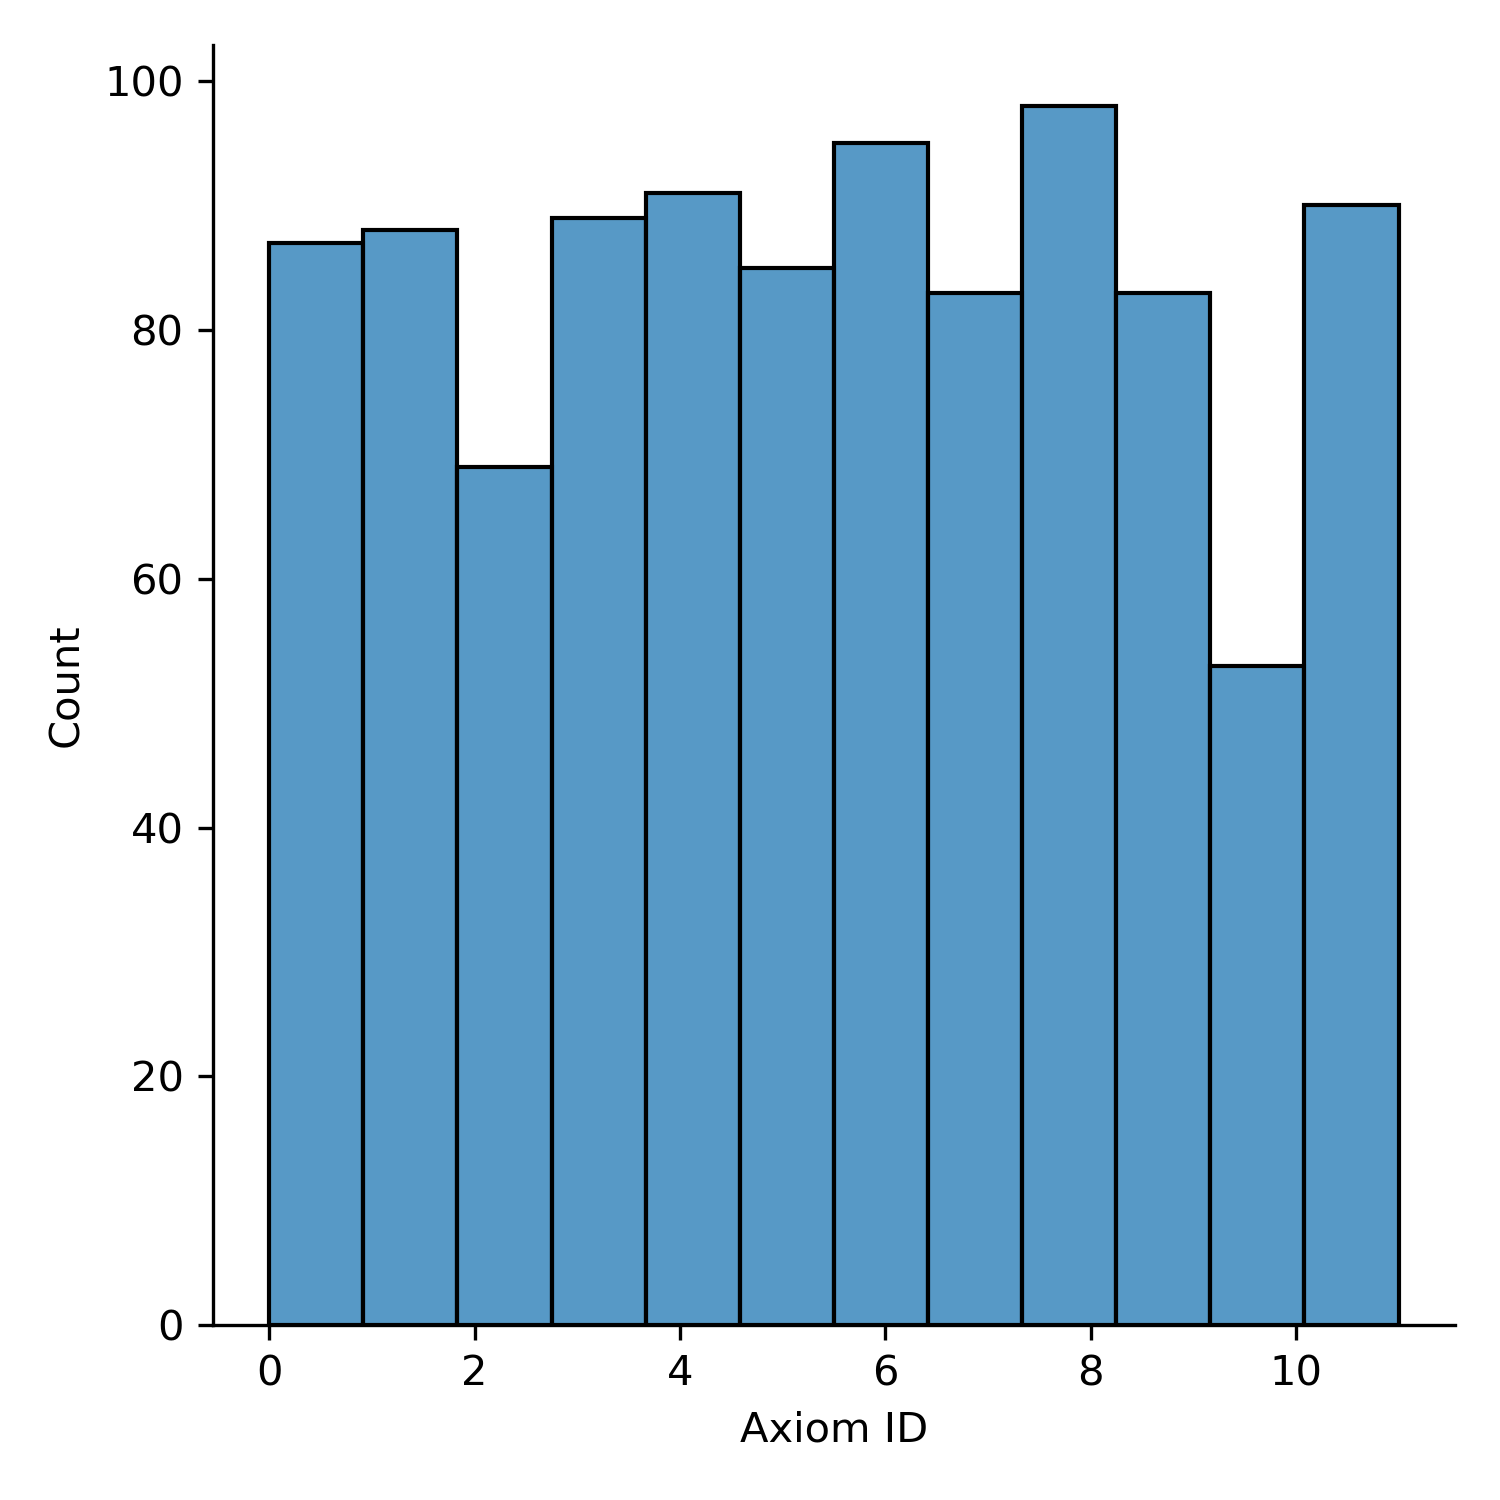
\includegraphics[width=\textwidth]{Axiom ID_2020-10-28--16-00-12.png}
		\caption{Axiom ID distribution}
	\end{subfigure}
	\hfill
	\begin{subfigure}[b]{0.45\textwidth}
		\centering
		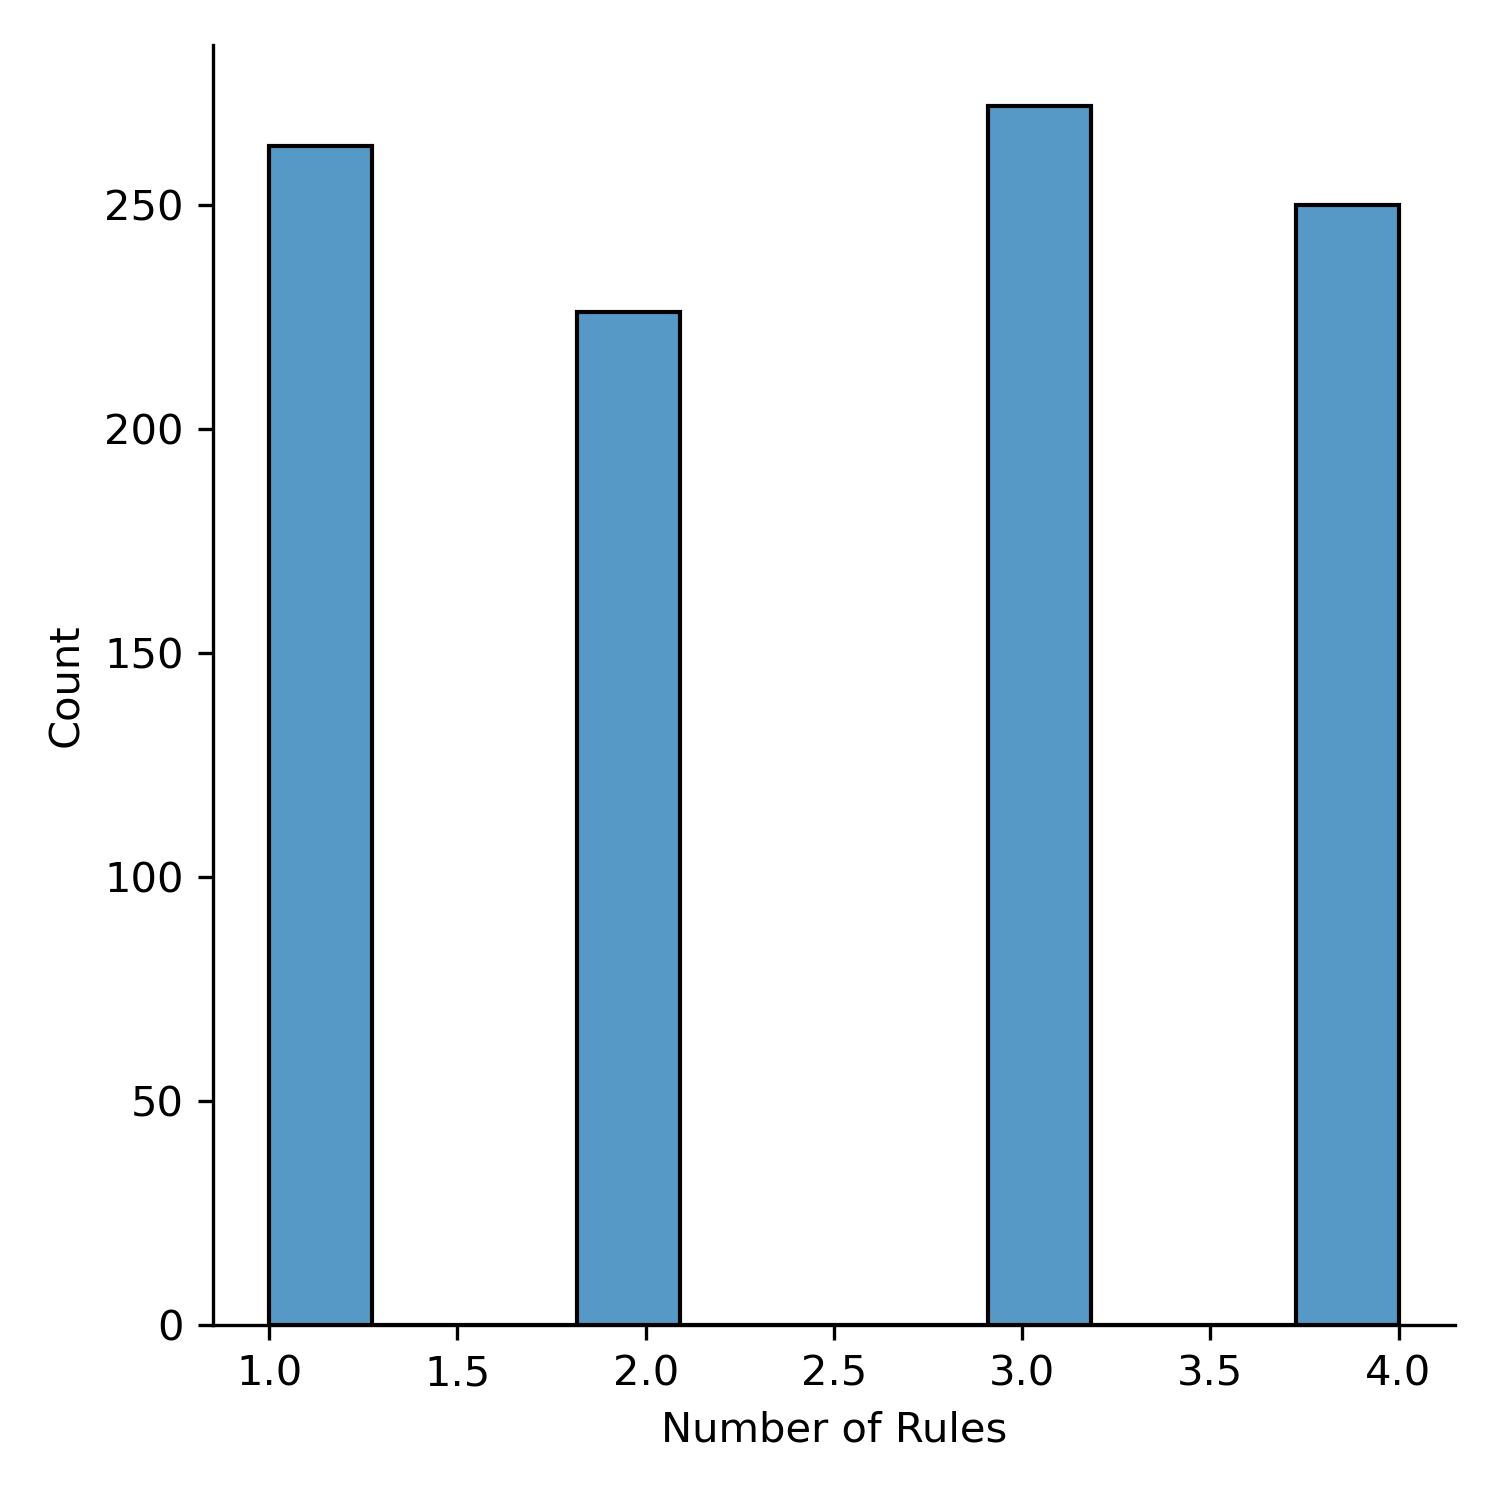
\includegraphics[width=\textwidth]{Number of Rules_2020-10-28--16-00-12.png}
		\caption{Number of rules distribution}
	\end{subfigure}
	\hfill
	\begin{subfigure}[b]{0.45\textwidth}
		\centering
		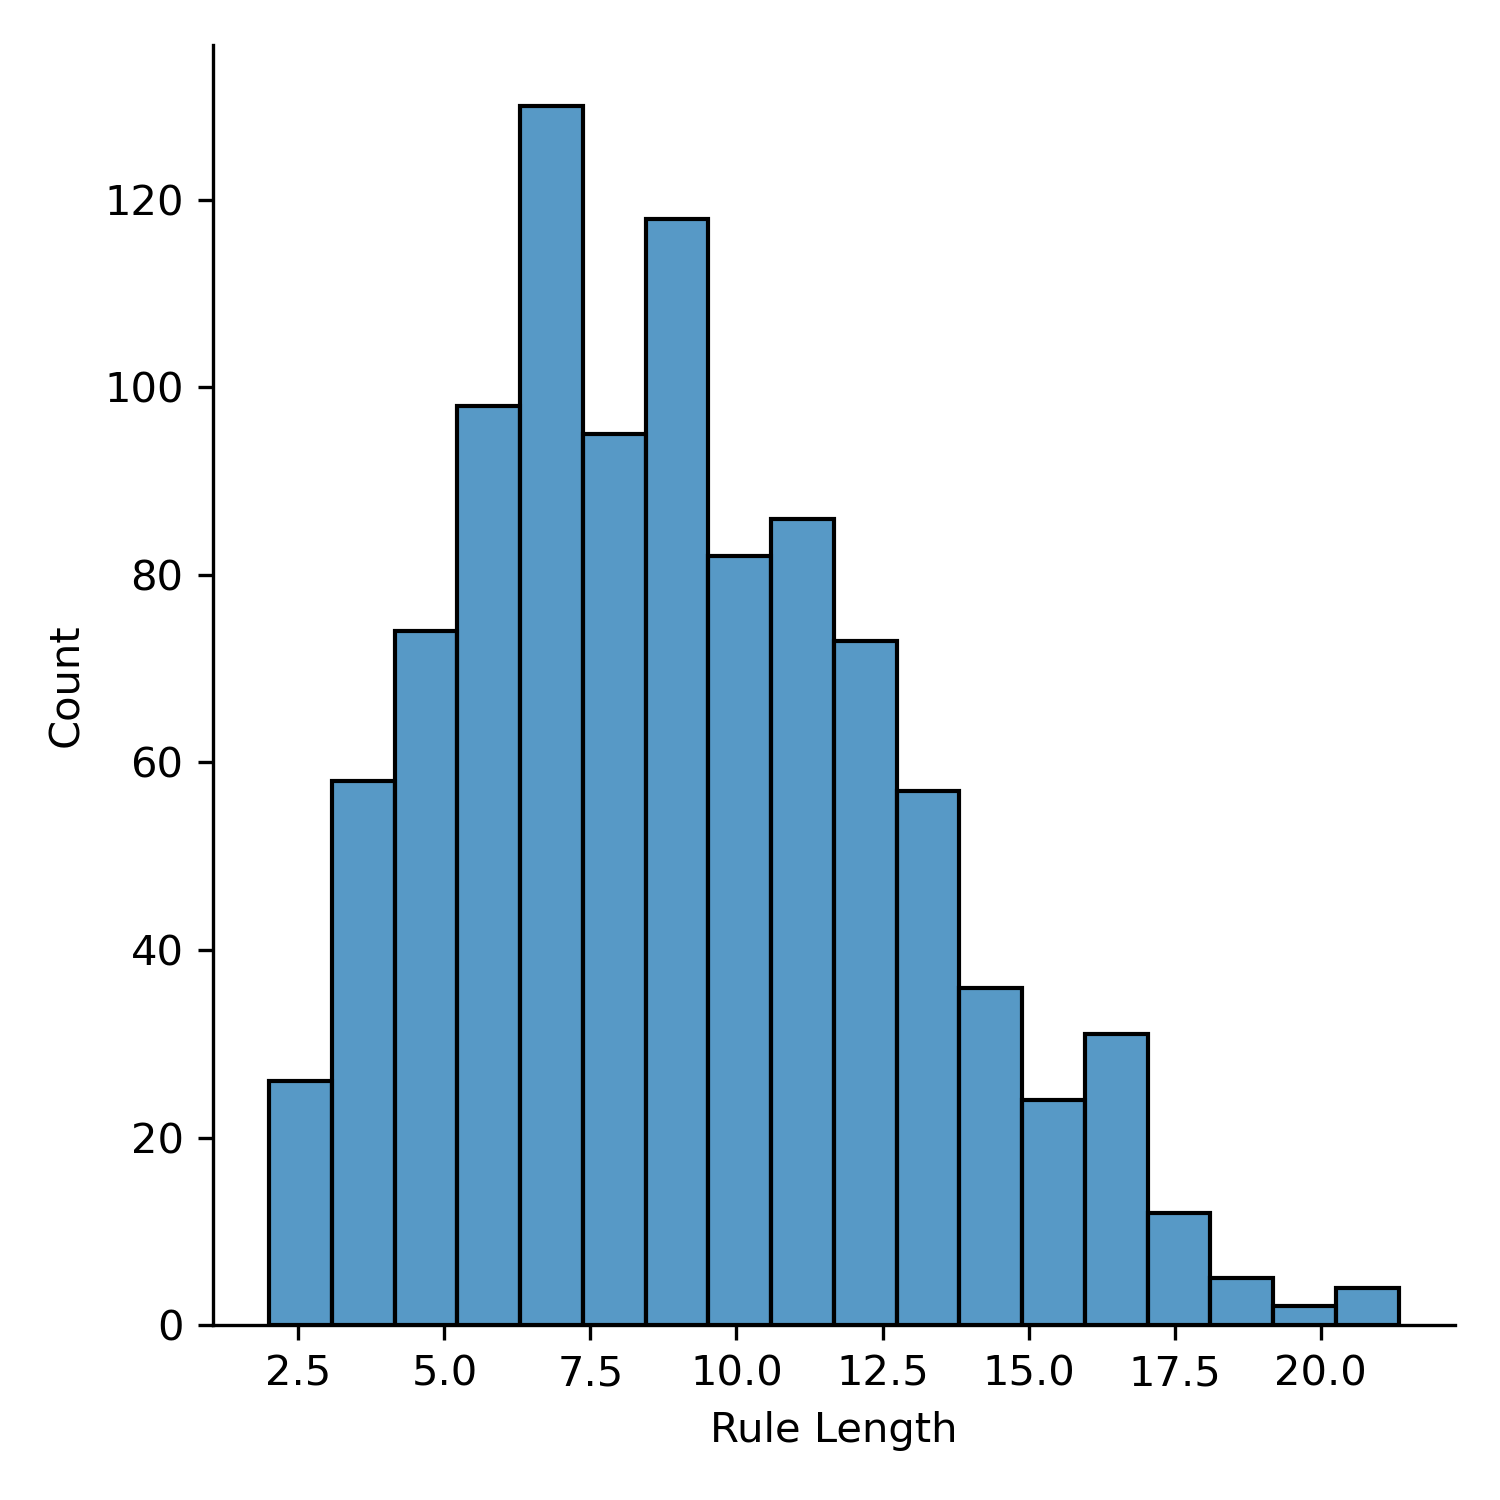
\includegraphics[width=\textwidth]{Rule Length_2020-10-28--16-00-12.png}
		\caption{Average rule length distribution}
	\end{subfigure}
	\hfill
	\begin{subfigure}[b]{0.45\textwidth}
		\centering
		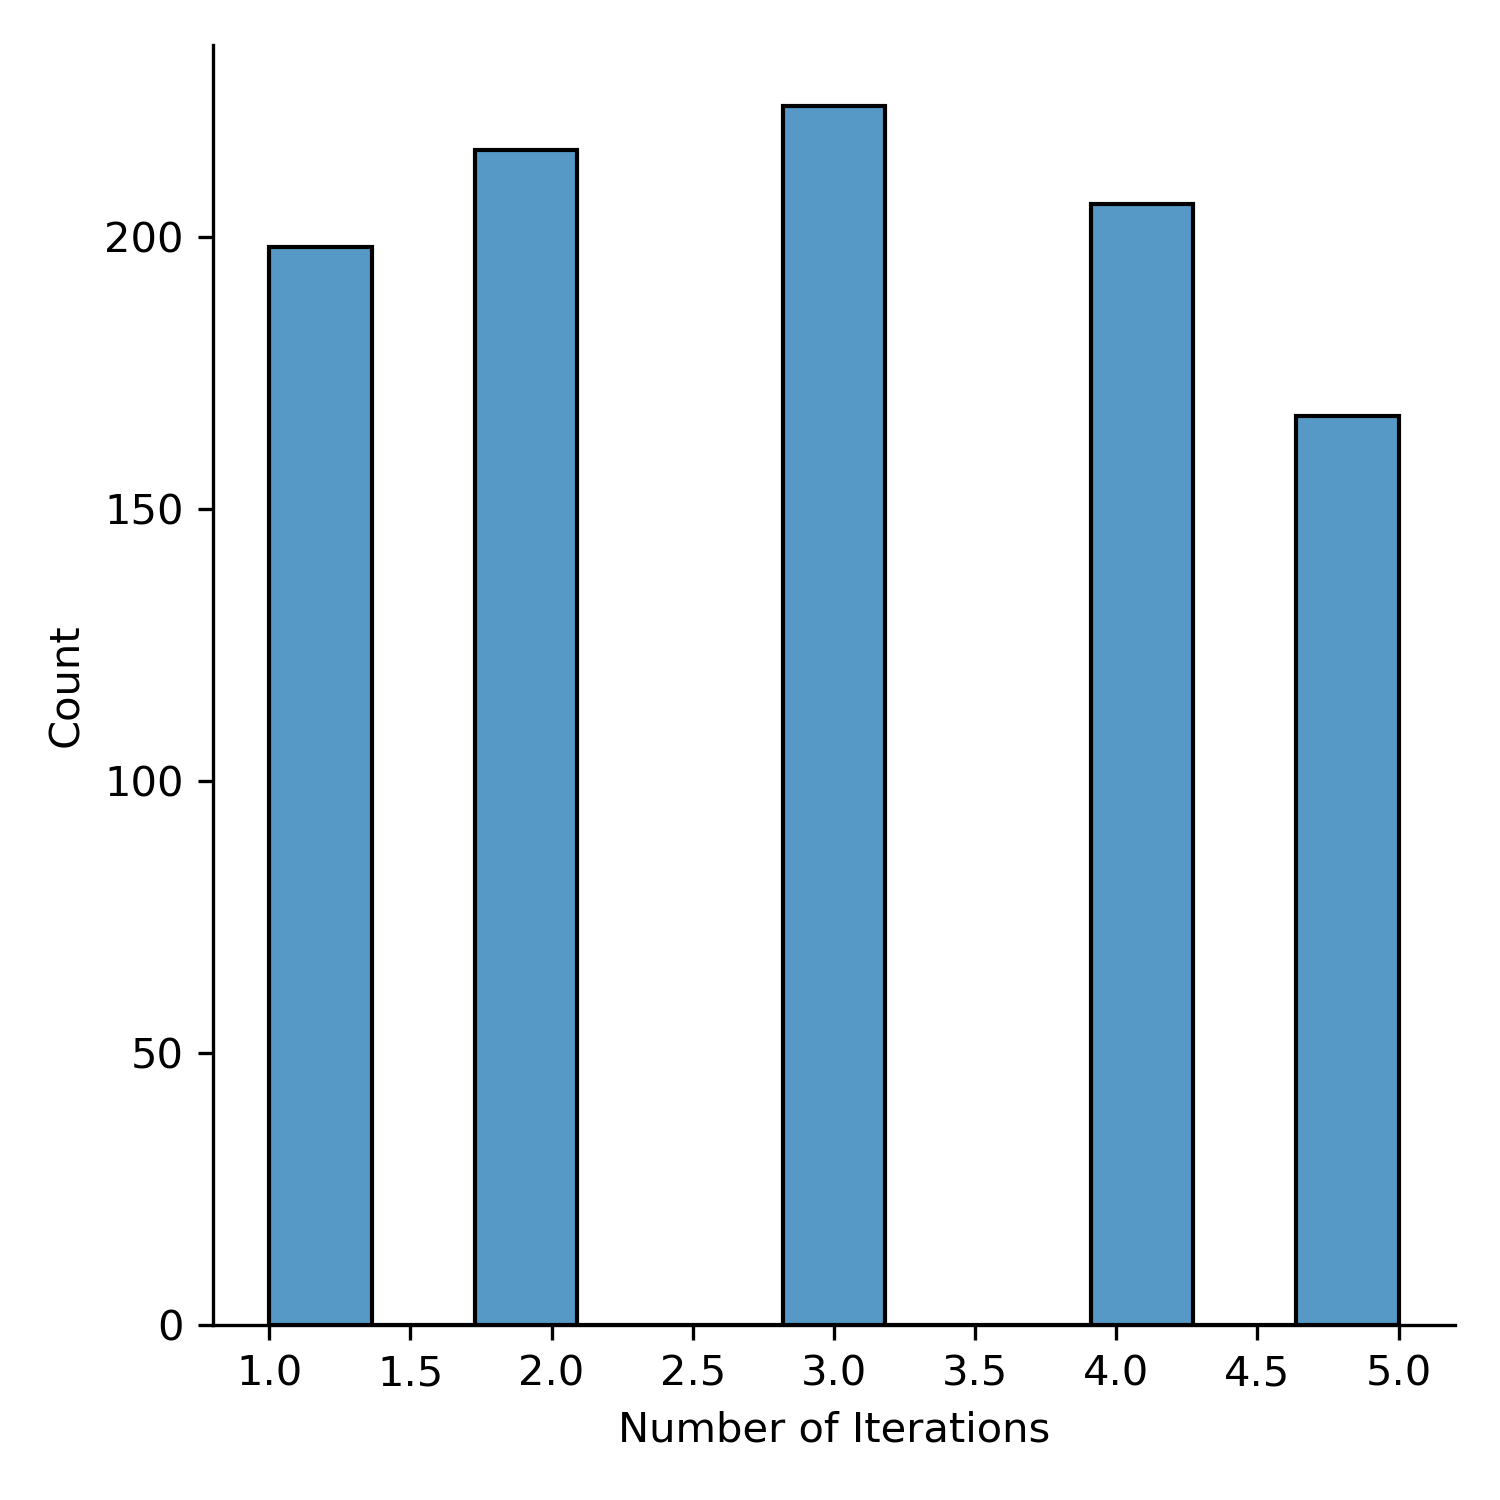
\includegraphics[width=\textwidth]{Number of Iterations_2020-10-28--16-00-12.png}
		\caption{Number of iterations distribution}
	\end{subfigure}
	\caption[L-System parameter distributions]{L-System parameter distribution histograms}
	\label{fig:lspardis}
\end{figure}

\subsection{CPPN Unit Generation}

Parameter ranges are outlined in Table~\ref{tab:cppnmc}.

% Please add the following required packages to your document preamble:
% \usepackage{booktabs}
\begin{table}[H]
\centering
\caption{CPPN unit generation parameters for a Monte Carlo analysis}
\label{tab:cppnmc}
\begin{tabular}{@{}lcc@{}}
\toprule
\multicolumn{1}{c}{\textbf{Parameter}} & \textbf{Minimum} & \textbf{Maximum} \\ \midrule
Seed                                   & 1                & 1000             \\
Model ID                               & 1                & N/A              \\
Scale                                  & 1                & N/A              \\
Number of hidden layers                & 2                & 10               \\
Size of the initial hidden layer       & 2                & 32               \\
Element removal threshold              & 0                & 100              \\ \bottomrule
\end{tabular}
\end{table}

\section{Scale Invariance}